\documentclass[12pt]{article}
\usepackage{graphicx}
\usepackage{longtable}
\usepackage{listings}
\usepackage[letterpaper, margin=2cm]{geometry}
\usepackage[T1]{fontenc}
\usepackage{polski}
\usepackage[export]{adjustbox}
\usepackage[utf8]{inputenc}
\usepackage[polish]{babel}
\graphicspath{{.}}
\usepackage{tocloft}
\usepackage{hyperref}

\hypersetup{%
    colorlinks,
    citecolor=black,
    filecolor=black,
    linkcolor=black,
    urlcolor=black
}

\renewcommand{\cftsecleader}{\cftdotfill{\cftdotsep}}

\lstset{
    postbreak=\mbox{\textcolor{red}{$\hookrightarrow$}\space}
    belowcaptionskip=1\baselineskip,
    breaklines=true,
    frame=L,
    numbers=left,
    xleftmargin=\parindent,
    language=bash,
    showstringspaces=false,
    basicstyle=\footnotesize\ttfamily,
    identifierstyle=\color{blue},
    stringstyle=\color{orange},
}

\begin{document}
    \centering
    
\includegraphics[width=5cm, height=5cm,]{herbPL.jpg}
    \hspace{2cm}
    
\includegraphics[width=5cm, height=5cm]{herbWEII.jpg}\\
    \vspace{2cm}
    {\Huge \textbf{SPRAWOZDANIE}}
    \vspace{2cm}
    \newline
    {\large PROGRAMOWANIE W CHMURZE OBLICZENIOWEJ}
    \vfill

    \raggedright{}

    \textbf{IMIĘ I NAZWISKO:} Piotr Czajka

    \textbf{NUMER LABORATORIUM} 7\\
    \textbf{GRUPA:} 7.1.2\\
    \textbf{Data wykonywania ćwiczenia:} 07.12.2018\\

    \newpage

    \tableofcontents{}

    \newpage

    \section{Cel laboratorium}
    Celem laboratorium było zapoznanie się z tworzeniem klastrów Swarm.

    \section{Przebieg ćwiczenia}

    \subsection{Zadanie pierwsze}

    Zainicjowano klaster swarm:

    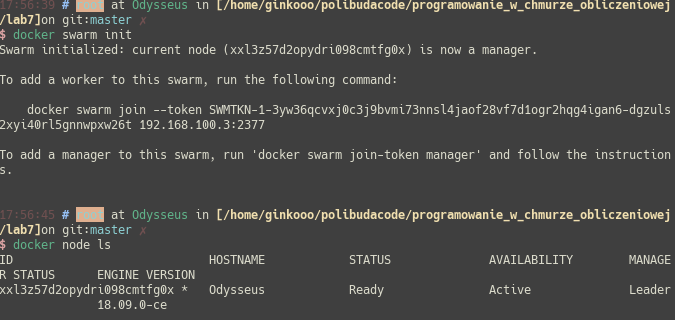
\includegraphics[width=\textwidth]{1_1.png}

    Stworzono i zweryfikowano działanie usługi w klastrze:

    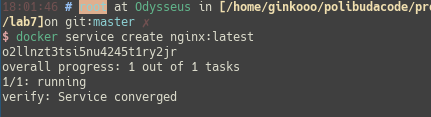
\includegraphics[width=\textwidth]{1_2.png}

    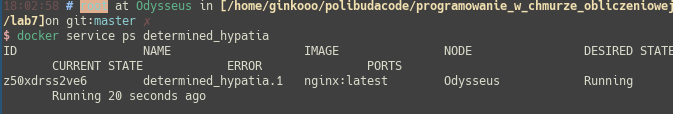
\includegraphics[width=\textwidth]{1_3.png}

    Jak widać tu, usługa działa na jednym kontenerze:

    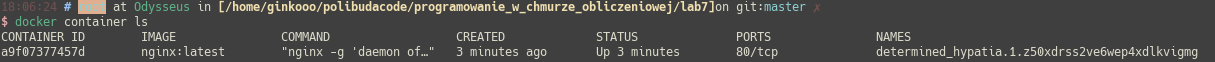
\includegraphics[width=\textwidth]{1_4.png}

    Tu skaluje usługę na 5 kontenerów:

    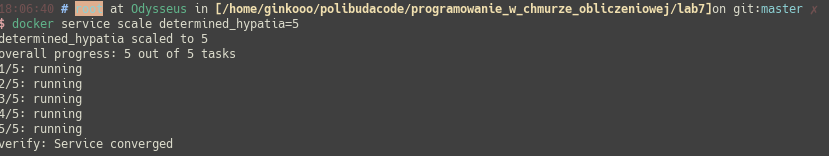
\includegraphics[width=\textwidth]{1_5.png}

    Wszystko działa na 5 kontenerach:

    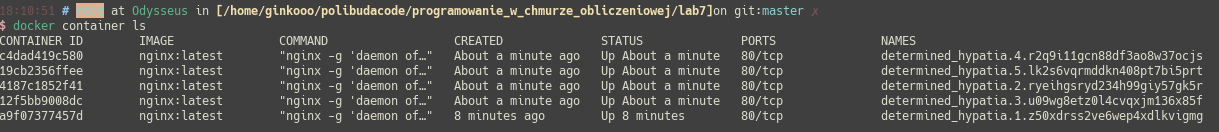
\includegraphics[width=\textwidth]{1_6.png}

    Symuluję awarię 3 z 5 kontenerów, usuwając je:

    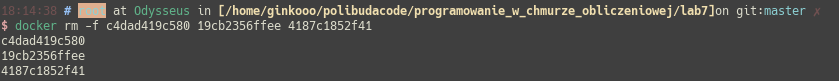
\includegraphics[width=\textwidth]{1_7.png}

    Tutaj widzimy, że Docker sam sobie stworzył nowe kontenery, w miejsce tych uszkodzonych (Można się zorientować po innym ID i któtkim uptime):

    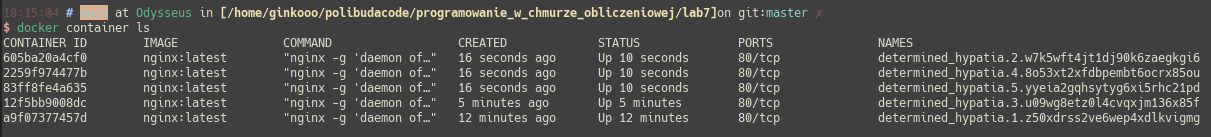
\includegraphics[width=\textwidth]{1_8.png}

    \subsection{Zadanie drugie}

    Stworzono następujące pliki w katalogu 'friendlyhello':

    app.py

    \lstinputlisting{friendlyhello/app.py}

    requirements.txt

    \lstinputlisting{friendlyhello/requirements.txt}

    Dockerfile

    \lstinputlisting{friendlyhello/Dockerfile}

    Połączono DockerHub z GitHub, a obraz jest zakolejkowany do budowania:

    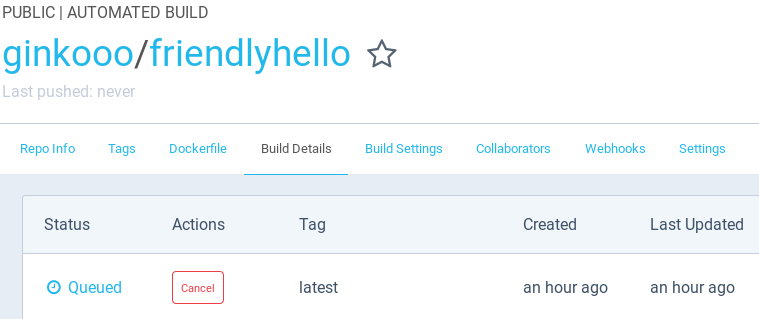
\includegraphics[width=\textwidth]{2_1.png}

    Link do githuba: github.com/ginkooo/friendlyhello

    Napisano taki oto docker-compose.yml:

    \lstinputlisting{docker-compose.yml}

    Uruchomiono stack 'myhello' na podstawie powyższego compose:

    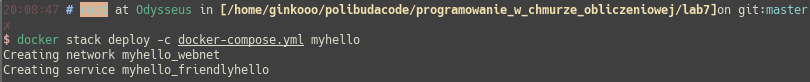
\includegraphics[width=\textwidth]{2_2.png}

    Tu widać, że stack jest uruchomiony:

    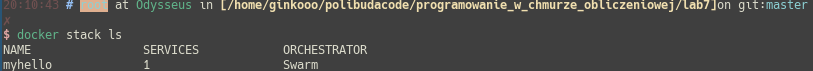
\includegraphics[width=\textwidth]{2_4.png}

    Sprawdzono w firefoxie, aplikacja działa:

    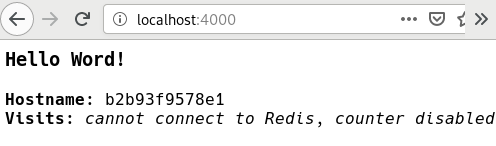
\includegraphics[width=\textwidth]{2_3.png}

    Tą komendą możemy przeskalować usługę do 7 replik

    Teraz odpytajmy serwer kilka razy:

    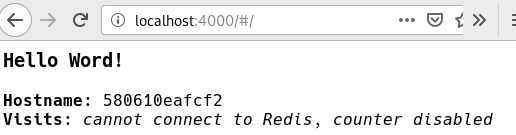
\includegraphics[width=\textwidth]{2_10.png}

    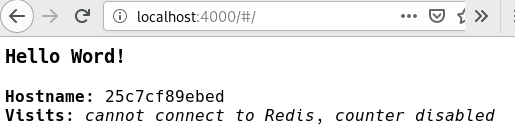
\includegraphics[width=\textwidth]{2_11.png}

    Rządania są dynamicznie oddelegowywane do różnych kontenerów je wykonujących. Efektem tego jest zmiana wartości w linijce Hostname.






\end{document}
